\documentclass[aspectratio=169]{beamer}
\setbeamertemplate{navigation symbols}{}
\usepackage{color,amsmath,comment, subfigure}
\usepackage{booktabs}
\def\vf{\vfill}
\usepackage{url}

%\setbeameroption{show notes}

%%%%%%%%%%%%%%%%%%%%%%%%%%
\title[]{Class 11: Cascades and fads in cultural markets}
\author[]{Matthew J. Salganik}
\institute[]{Sociology 204: Social Networks\\Princeton University}
\date[]{
2/2: Self-fulfilling prophicies
\vfill

\begin{flushleft}
\vspace{0.6in}

\includegraphics[width=0.1\textwidth]{figures/cc.png}
\end{flushleft}

}

\note{
Next year possibly have them predict experiment 3 which they have not seen
}

\begin{document}
%%%%%%%%%%%%%%%%%%%%%%%%%%%
\frame{\titlepage}
%%%%%%%%%%%%%%%%%%%%%%%%%%%
\begin{frame}

\begin{columns}
   \column{0.35\textwidth}
    \begin{block}{}
      
\includegraphics[width=\textwidth]{figures/vise}
    \end{block}

   \column{0.6\textwidth}
     \begin{block}{}
       Someone bought and returned 17,000 copies of this book.
       \pause
       It was David Vise.\\
     \end{block}
  \end{columns}

\end{frame}
%%%%%%%%%%%%%%%%%%%%%%%%%%%%%%%%%%%%%%%%%%%%

\begin{frame}
\frametitle{Self-fulfilling prophecies}

``[a] self-fulfilling prophecy is, in the beginning, a {\em false}
definition of the situation evoking a new behavior which make the
originally false conception come {\em true}.'' Robert Merton (1948)\\

\vspace{0.3in}
Vise's book sold more than 180,000 copies.  How much of this was
due to a self-fulfilling prophecy?  Hard to say.

\vspace{0.3in} 
Again, this is difficult with observational data, but possible with a multiple-realization experiment

\end{frame}

%%%%%%%%%%%%%%%%%%%%%%%%%%%%%%%%%%%%%%%%%%%%%
\begin{frame}
\frametitle{Experimental design}

\begin{figure}
  \centering
  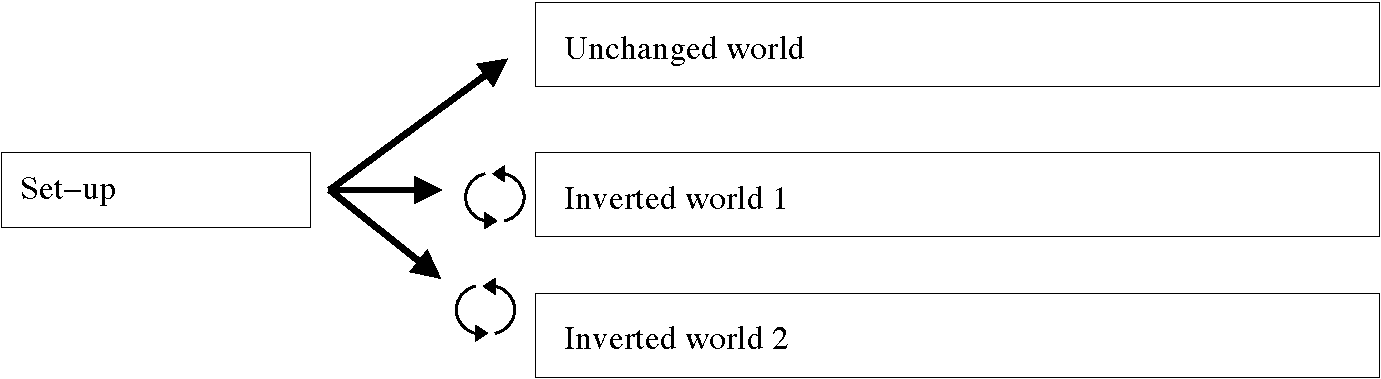
\includegraphics[width=0.8\textwidth]{figures/exp34_asaslides}
\end{figure}

\end{frame}
%%%%%%%%%%%%%%%%%%%%%%%%%%%%%%%%%%%%%%%%%%%%%%%%%%%%%%%%
\begin{frame}
\frametitle{Tracking song 1 and song 48}

\begin{figure}
  \centering
  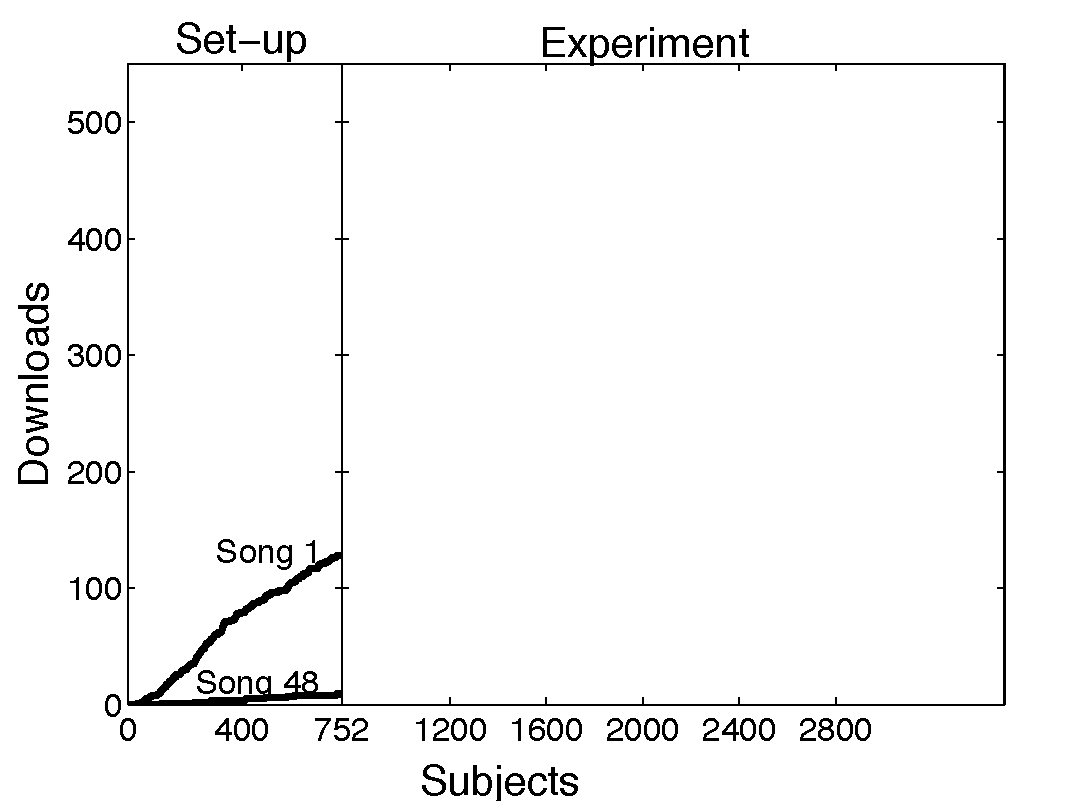
\includegraphics[width=0.7\textwidth]{figures/pair1_34_asa1}
\end{figure}

\end{frame}
%%%%%%%%%%%%%%%%%%%%%%%%%%%%%%%%%%%%
\begin{frame}
\frametitle{Tracking song 1 and song 48}

\begin{figure}
  \centering
  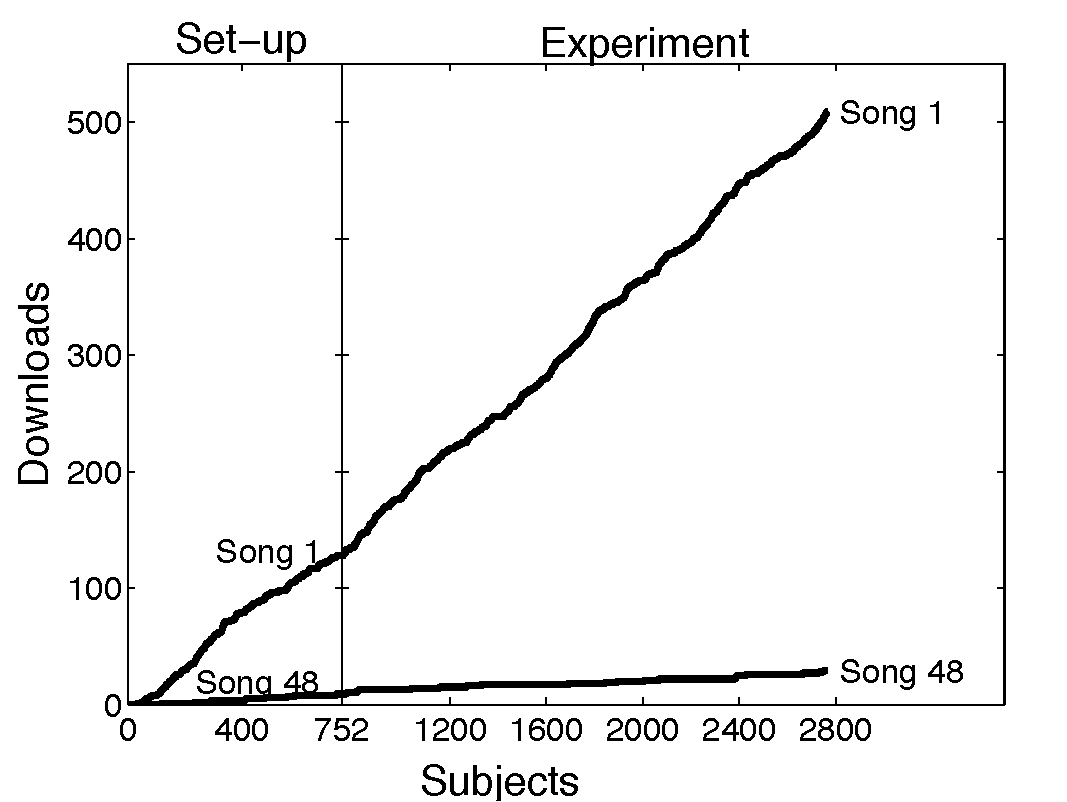
\includegraphics[width=0.7\textwidth]{figures/pair1_34_asa2}
\end{figure}

\end{frame}
%%%%%%%%%%%%%%%%%%%%%%%%%%%%%%%%%%%%
\begin{frame}
\frametitle{Tracking song 1 and song 48}

\begin{figure}
  \centering
  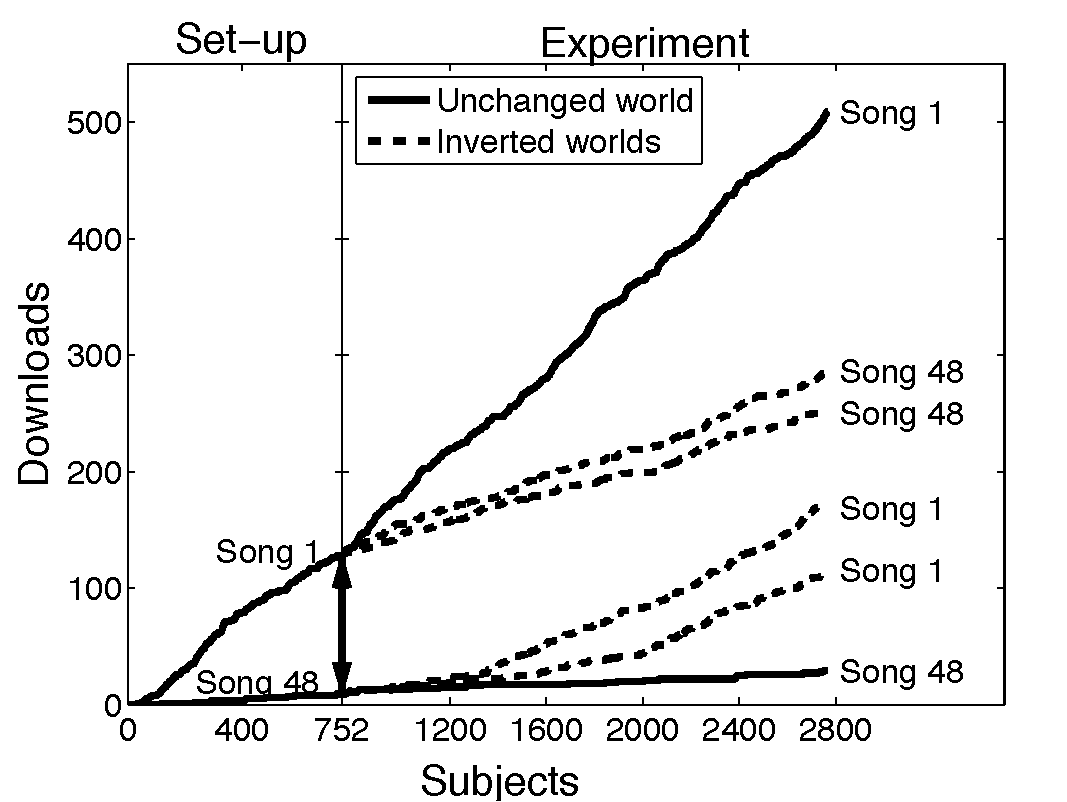
\includegraphics[width=0.7\textwidth]{figures/pair1_34_asa3}
\end{figure}

\end{frame}
%%%%%%%%%%%%%%%%%%%%%%%%%%%%%%%%%%%%
\begin{frame}
\frametitle{Tracking song 2 and song 47}

\begin{figure}
  \centering
  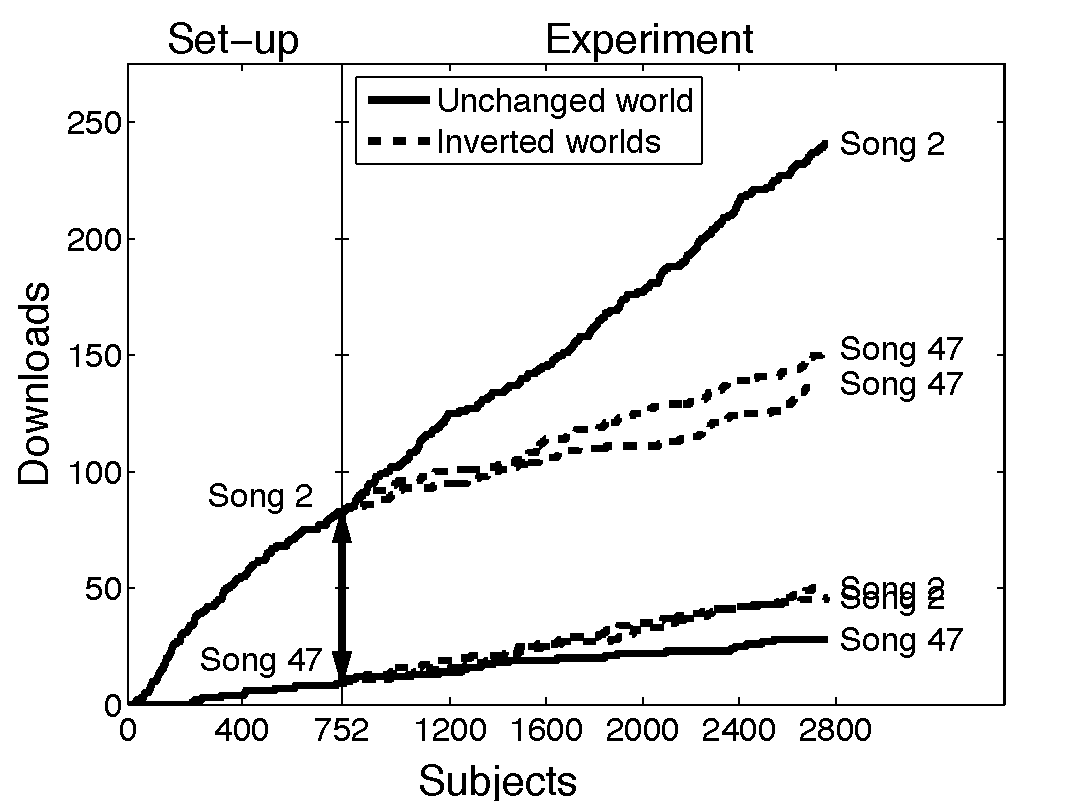
\includegraphics[width=0.7\textwidth]{figures/pair2_34_asa}
\end{figure}

\end{frame}
%%%%%%%%%%%%%%%%%%%%%%%%%%%%%%%%%%
\begin{frame}

\begin{figure}
  \centering
  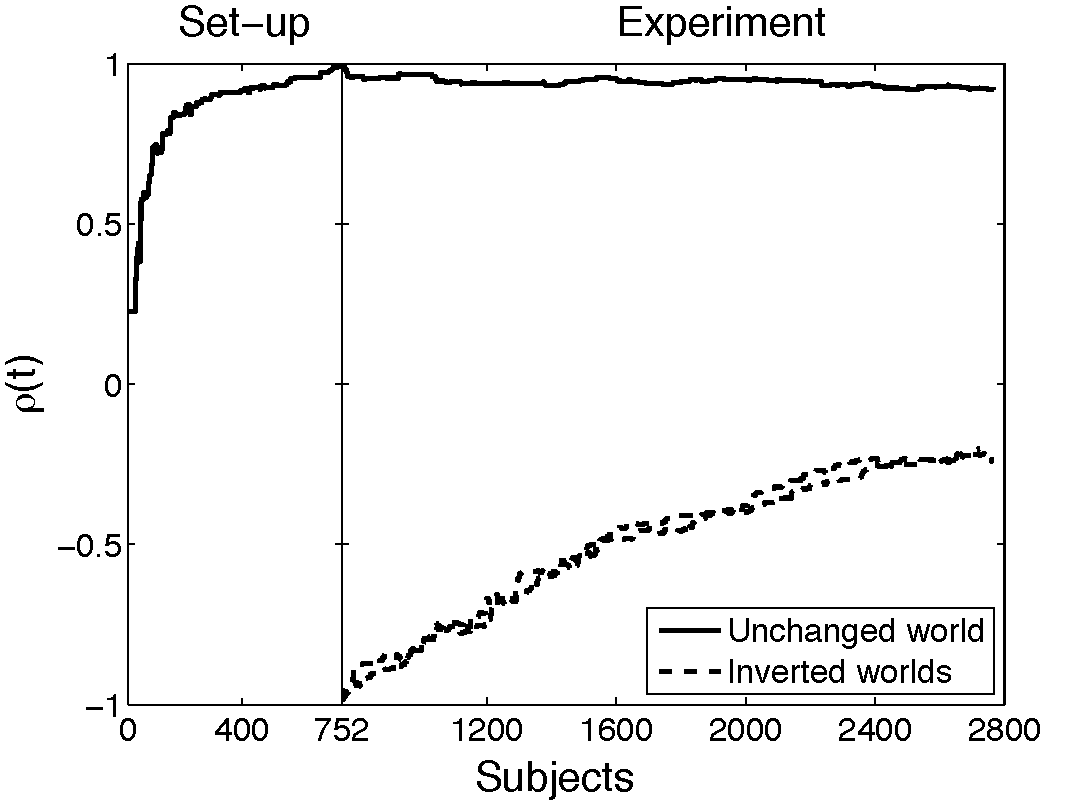
\includegraphics[width=0.8\textwidth]{figures/dynamics_rankcorr_exp3_v34_nolabel}
\end{figure}

\end{frame}
%%%%%%%%%%%%%%%%%%%%%%%%%%%%%%%%%%
\begin{frame}

\begin{figure}
  \centering
  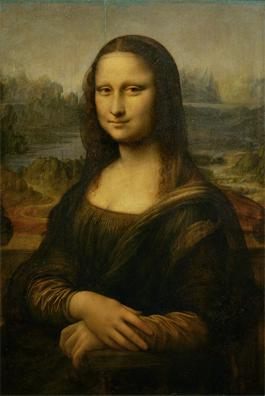
\includegraphics[height=0.8\textheight]{figures/monalisa}
\end{figure}

\end{frame}
%%%%%%%%%%%%%%%%%%%%%%%%%%%%%%
\begin{frame}

\begin{columns}[b]
  \column{0.3\textwidth}
  \begin{figure}
    \centering
    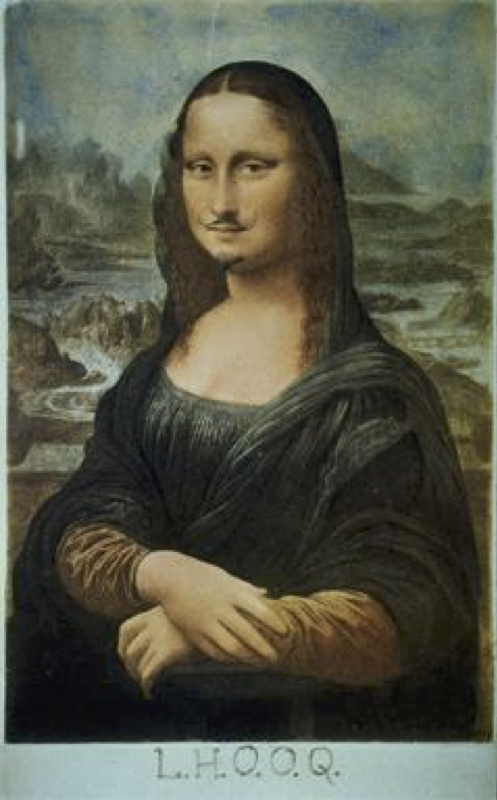
\includegraphics[height = 1.8in]{figures/monalisa_duchamp}
  \end{figure} 
  \begin{center} 
  (Duchamp, 1919)
  \end{center}

\pause

  \column{0.3\textwidth}
  \begin{figure}
    \centering
    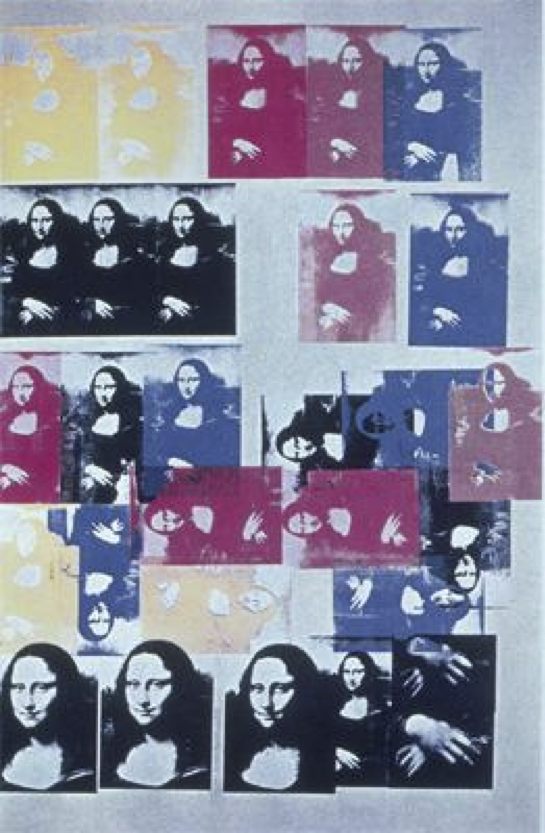
\includegraphics[height = 1.8in]{figures/monalisa_warhol}
  \end{figure} 
  \begin{center}
  (Warhol, 1963)
  \end{center}

\pause

  \column{0.3\textwidth}
  \begin{figure}
  \centering
  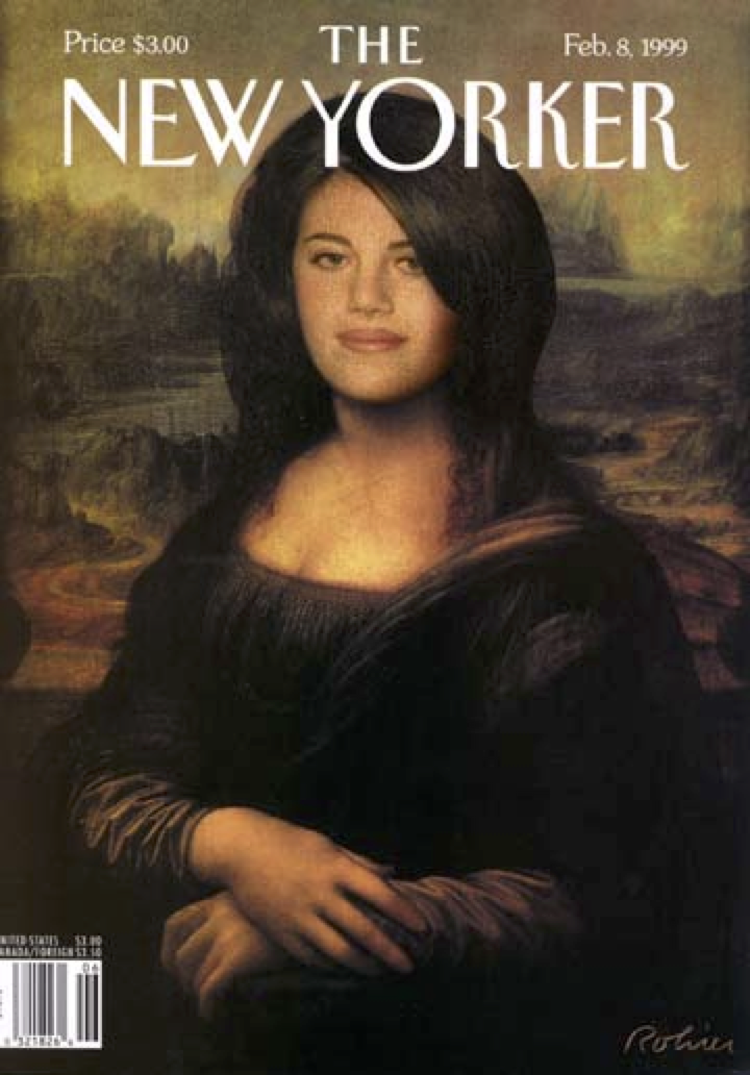
\includegraphics[height = 1.8in]{figures/monalisa_newyorker}
  \end{figure}
  \begin{center}
  (Roher, 1999)
  \end{center}
\end{columns}

\end{frame}

%%%%%%%%%%%%%%%%%%%%%%%%%%%%%%%%%%
\begin{frame}

\begin{figure}
  \centering
  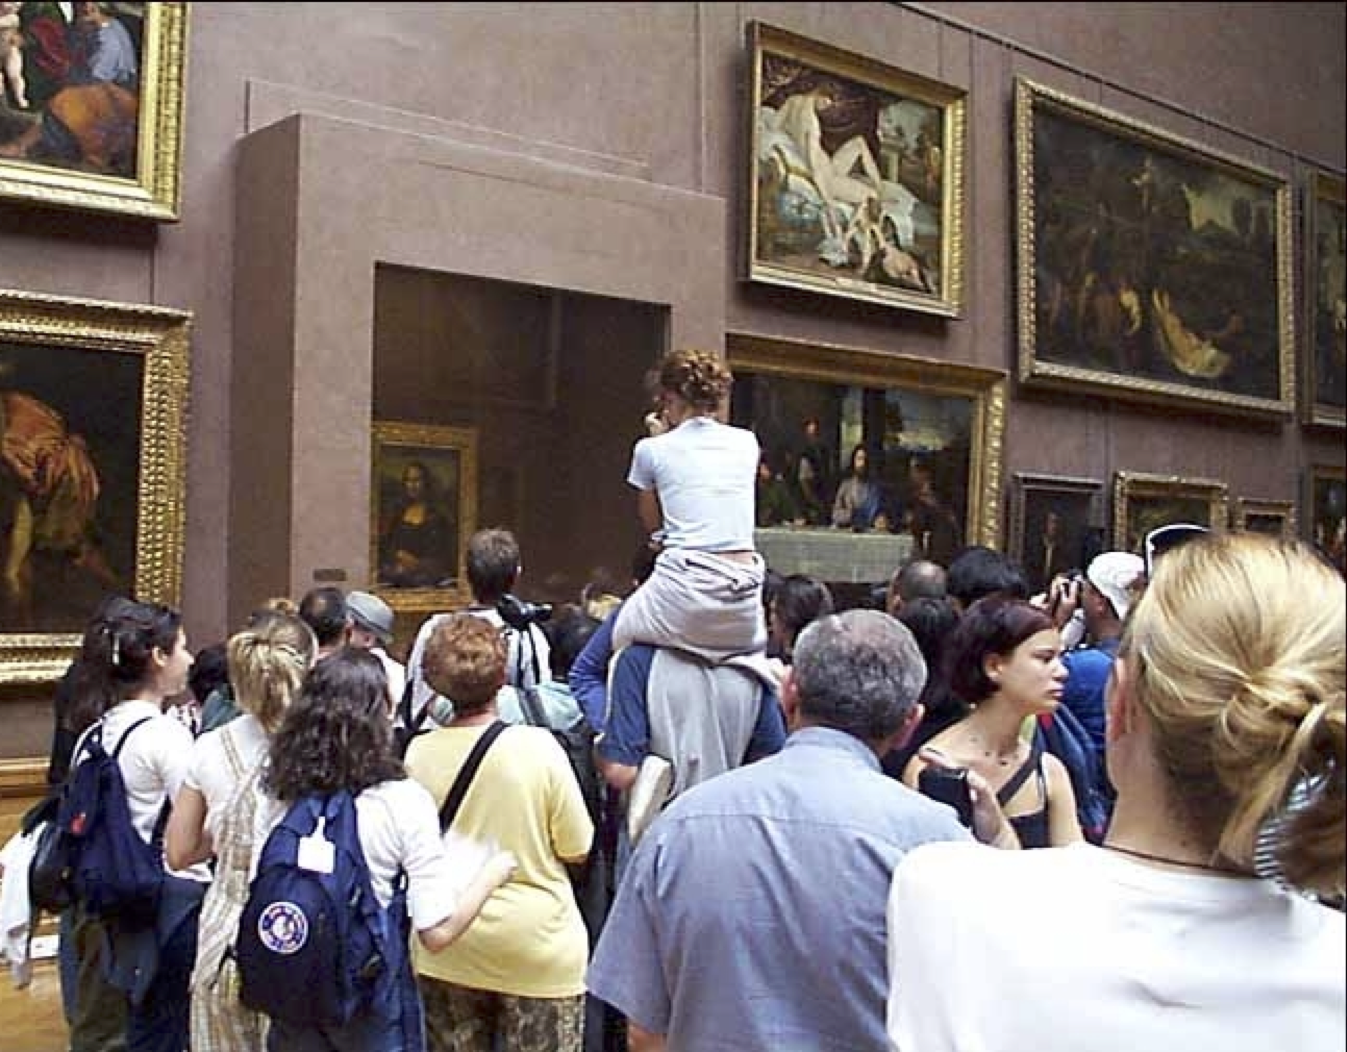
\includegraphics[width=0.7\textwidth]{figures/monalisa_onshoulders_cut3}
\end{figure}

\end{frame}
%%%%%%%%%%%%%%%%%%%%%%%%%%%%%%%%%
\begin{frame}

Summary:
\begin{itemize}
\item social influence can lead to inequality and unpredictability of success
\pause
\item social influences weakens the relationship between appeal and success
\pause
\item you can predict failure but you can't predict success
\pause
\item the perception of success can become a self-fulfilling prophecy
\pause
\end{itemize}

Download all the data from these experiments: \url{http://opr.princeton.edu/archive/cm/}

\end{frame}
%%%%%%%%%%%%%%%%%%%%%%%%%%
\begin{frame}

Next steps:
\begin{itemize}
\item please fill out the after lecture survey
\pause
\item good luck on the midterm
\pause
\item have a wonderful and safe spring break
\end{itemize}

\end{frame}
%%%%%%%%%%%%%%%%%%%%%%%%%%

\end{document}
